%!TEX root = ../report.tex
\documentclass[../report.tex]{subfiles}

\begin{document}
    \section{Methodology}
    \label{sec:methodology}

    % Describe all conceptual details about your approach in this section.
    % Add any necessary subsections to improve the presentation.

    % Feel free to rename this section to better reflect the concrete topic you are discussing.
    \subsection{Simulation Framework}
    A set of simulation frameworks was investigated to select the best simulation that is available for the project. Gazebo was selected as the simulation based on its compatibility with ROS2 
    and the availability of the plugins that are already made available due to the familiarity of the platform. The SJTU drone system was selected as the drone model for the simulation as it was 
    lightweight and also easy to work with. A new radiation sensor plugin and radiation source plugin were developed to simulate the radiation source and the sensor. This plugin can be easily 
    integrated into the simulation and can be used to simulate the radiation source and the sensor. 
        
    To accurately represent realistic radiation behavior, the radiation source is modeled as a point gamma radiation source that emits radiation uniformly in all directions. The radiation sensor 
    receives and publishes data in the form of photon count rates; however, this count rate is subject to attenuation caused by trees and the air surrounding the sensor. 

    The attenuation from trees is implemented through ray tracing, which helps to determine if the sensor has a clear line of sight to the radiation source. If trees obstruct the line of sight, 
    the radiation is attenuated based on the type of tree and a specific attenuation factor. The positions of the trees are generated dynamically according to the map size, while ensuring a 
    maintained specific distance between each tree.
        
    % \subsection{Measurement Model}

    % with measurement model:

    % % mt = Σ(i,j∈Ω) [b(i,j)/((x-xi)^2 + (y-yj)^2 + h^2)] + N(0, 0.5mt)
    % \begin{equation}
    %     m_t = \sum_{i,j \in \Omega} \left[ \frac{b(i,j)}{(x - x_i)^2 + (y - y_j)^2 + h^2} \right] + N(0, 0.5m_t)
    % \end{equation}

    \subsection{Evaluation Framework}

    A new interface for handling the simulation and experiment metrics was developed. The interface is designed with PyQt5, a Python library for creating graphical user interfaces. 
    Two interfaces have been developed that allow one to either handle all the parameters in the workspace or visualize any number of algorithms running within the workspace.
        
    \subsubsection{Parameter Editor}
    The parameter editor application serves multiple purposes beyond the current project. It was developed to provide a unified interface that consolidates all configuration files in YAML format. 
    To ensure compatibility with ROS2 packages, the interface can load the names of the ROS2 packages of interest from a YAML file. This file is then processed to identify which packages should be
     searched for within the root of the ROS2 workspace. The identified YAML files are sorted according to the package or workspace in which they were found, allowing the user to select the 
     package of interest. Once selected, the YAML files are loaded and displayed in a tabular format. This interface enables the users to add, remove and save changes to the YAML files.  

    Another feature of this interface is its ability to identify common parameters shared across different algorithms. These parameters can include the search area, source location, ROS2 
    topic names, and more. Changes made in this section of the application are applied to all instances of the same parameters across the project workspace. This functionality enables users 
    to transition or migrate the project to different simulation frameworks or configurations with varying parameters.

    \subsubsection{Evaluation Visualizer}

    Each algorithm, upon successful completion, is saved in a standardized JSON file format. All metrics contained in these files are consistent across all algorithms, which facilitates easier 
    comparison and visualization of the results.

    The Evaluation Visualizer is an interface designed to visualize these results based on a set of configurations. When the interface is opened, the user can select the input directory containing 
    the saved JSON files, followed by a directory where the evaluated files will be saved. Once the input directory is selected, the interface loads all JSON files and categorizes them by algorithm
    name. From this interface, users can specify the number of experiments to be evaluated from the total runs. After processing the analysis, the results of the algorithm runs are evaluated and 
    displayed in the next tab, with a copy saved locally for future visualization.

    The algorithms are assessed together based on predefined performance metrics, and various plots representing additional metrics from the runs are generated along with a report taht tabulates 
    the evaluation results for each algorithm. 

    This interface also comes with an extra tab that gives the option to generate different types of plots based on the metrics that can be selected for both the x and y-axis. The corresponding 
    plot will be generated and displayed within the same window.

    This application additionally provides a feature to do statistical analysis on the results. The users can select the metrics they want to perform the analysis on, and this will generate a 
    statistical analysis report that can be read and interpreted by the user.

    \subsection{Algorithms}
    \subsubsection{Information-Gain-based Algorithm}

    The proposed method combines a particle filter for sequential Bayesian estimation with information-driven observer control using Rényi divergence. The particle filter approximates
    the joint posterior density of the source parameters through a set of weighted particles, while Rényi divergence guides measurement collection to maximize information gain. 
    This method operates in two distinct phases: an initial exploration phase and an information-driven exploitation phase. Unlike previous approaches that use Fisher information for observer control
    after detection \cite{Ristic2007AnIG}, this method uses Rényi divergence throughout both phases. This choice is motivated by ability of Rényi divergence to enable optimal measurement collection 
    by considering the complete probability density function rather than just parameter estimates.

    \paragraph{Particle Filter Framework}
    The source state $X = [x, y, I]^T$ comprises 2D position $(x,y)$ and intensity $I$. The posterior distribution is approximated using weighted particles:

    \begin{equation}
    p(X|z_{1:k}) \approx \sum_{i=1}^N w_k^i \delta(X - X_k^i)
    \end{equation}

    where $X$ is the state vector containing position and intensity, $z_{1:k}$ represents all measurements up to time $k$, $w_k^i$ is the normalized weight of particle $i$, $N$ is the total number 
    of particles, $\delta(\cdot)$ is the Dirac delta function

    The radiation measurement model incorporates inverse square law decay and atmospheric attenuation:

    \begin{equation}
    \lambda(X, x_k) = \left(\frac{I}{d^2(x_k, X)} + \mu_b\right)\tau_k \cdot \exp(-\beta d(x_k, X))
    \end{equation}

    where, $\lambda(X, x_k)$ is the expected measurement rate at position $x_k$, $I$ is the source intensity, $d(x_k, X)$ is the distance from measurement position to source, $\mu_b$ is the 
    background radiation rate, $\tau_k$ is the measurement exposure time, $\beta$ is the atmospheric attenuation coefficient.

    \paragraph{Two-Phase Search Strategy}
    During the exploration phase, the detection probability is monitored using:

    \begin{equation}
    P(\text{detection}|z_k) = \frac{r_k}{1 + r_k}, \quad r_k = \frac{\frac{1}{N}\sum_{i=1}^N P(z_k|X_k^i)}{P(z_k|\text{background})}
    \label{eq:prob_detection}
    \end{equation}

    where, $P(\text{detection}|z_k)$ is the probability of source presence, $r_k$ is the likelihood ratio, $P(z_k|X_k^i)$ is the measurement likelihood for particle $i$, $P(z_k|\text{background})$ 
    is the background-only likelihood.

    In the exploitation phase, measurement locations are optimized using Rényi divergence:

    \begin{equation}
    D_\alpha(x_k') = \frac{1}{\alpha-1} \log\left(\frac{g_\alpha(x_k')}{g_1(x_k')^\alpha}\right) \cdot E(x_k')
    \end{equation}

    with:
    \begin{equation}
    g_\alpha(x_k') = \frac{1}{N}\sum_{i=1}^N \exp(\alpha \hat{z}_k^i)
    \end{equation}

    where, $D_\alpha(x_k')$ is the Rényi divergence for candidate position $x_k'$, $\alpha$ is the Rényi divergence parameter ($\alpha > 0$), $g_\alpha(x_k')$ is the $\alpha$-weighted prediction 
    sum, $\hat{z}_k^i$ is the normalized predicted measurement, $E(x_k')$ is the exploration bonus term. 

    Rényi divergence generalizes mutual information and provides a measure of how well a candidate measurement position $x_k'$ can distinguish between the current posterior distribution of the source state and a uniform or background distribution.

    \paragraph{Sequential State Estimation}
    The particle weights are updated using:

    \begin{equation}
    w_k^i = \frac{\tilde{w}_k^i}{\sum_{j=1}^N \tilde{w}_k^j}
    \end{equation}

    with unnormalized weights:
    \begin{equation}
    \tilde{w}_k^i = w_{k-1}^i \cdot \exp(\log L_k^i - \max_j \log L_k^j) \cdot c_k^i
    \end{equation}

    where, $w_k^i$ is the normalized weight of particle $i$ at time $k$, $\tilde{w}_k^i$ is the unnormalized weight, $L_k^i$ is the measurement likelihood for particle $i$, $c_k^i$ is the geometric 
    consistency term. The geometric consistency term $c_k^i$ evaluates how well each particle explains the measurement patterns obtained from different observation angles, complementing the circular 
    measurement strategy used for position selection. This circular measurement pattern is particularly significant as demonstrated by Ristic et al. \cite{Ristic2007AnIG}, who in their first 
    method showed that measuring in a circle around the estimated source position helps discriminate the true source location, since getting too close to the source can result in higher 
    measurement uncertainty and estimation errors due to the inverse square law behavior of radiation.

    This framework enables efficient source detection and localization by combining systematic exploration with information-driven measurement optimization. The particle filter handles the non-linear measurement model while maintaining uncertainty estimation throughout the process.

    \begin{figure}[ht]
        \centering
        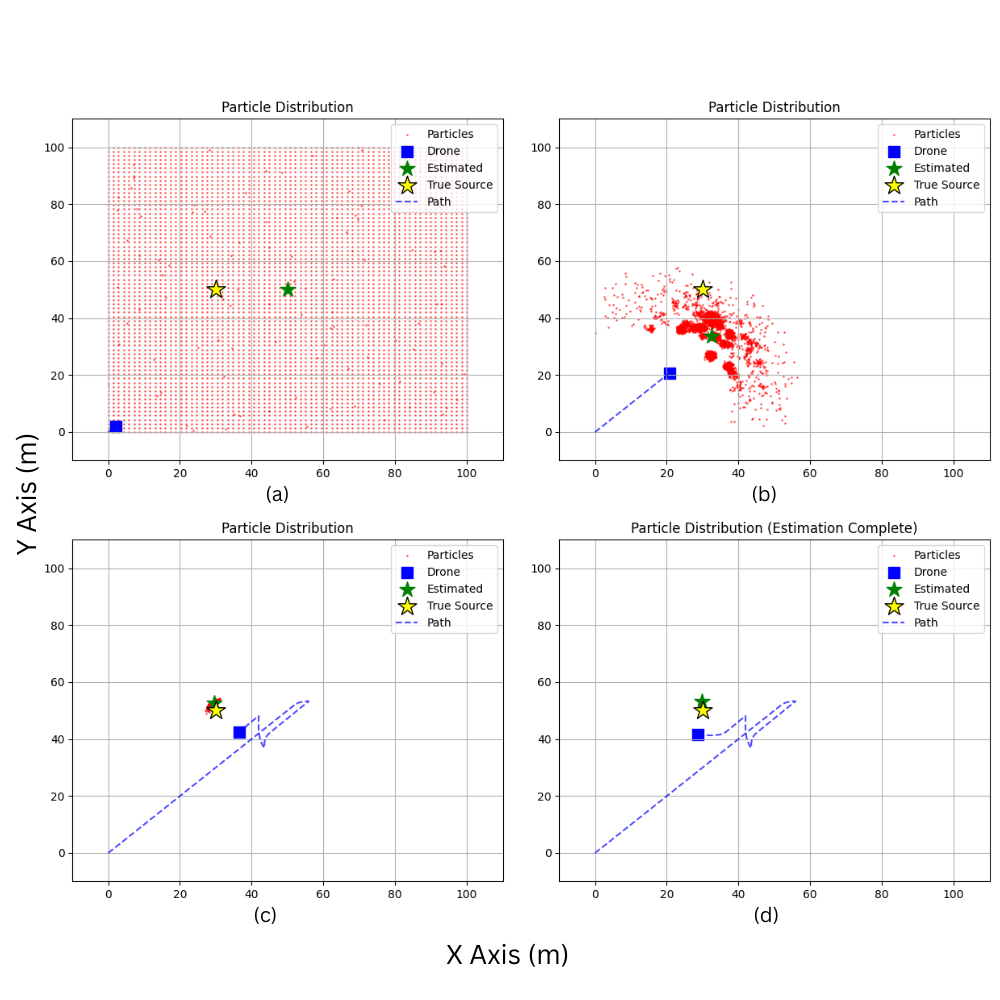
\includegraphics[width=\linewidth]{figures/entropy_algorithm_with_label.png}
        \caption{Information gain-based radiation source localization for source location (30, 50): a. Initial particle distribution across search area, 
        b. Particle resampling on source detection, 
        c. Convergence of particles near true source location, and 
        d. Final source position estimation with completed path}
        \label{fig:entropy_algorithm_with_plot}
    \end{figure}

    Figure~\ref{fig:entropy_algorithm_with_plot} represents the run of the information gain-based radiation source localization algorithm for a source located at (30, 50). The 
    particles are uniformly distributed across the search area initially, and the algorithm converges on the true source location after the source has been detected using ~\ref{eq:prob_detection} starting 
    from figure~\ref{fig:entropy_algorithm_with_plot}.b. The final source location theoretically is the point where the  particles converge as in figure~\ref{fig:entropy_algorithm_with_plot}.d.This 
    run localized the source at a distance of 3 meters from the actual source location.
    [ADD RESAMPLING AND UPDATE MECHANISM]


    \subsubsection{Rollout-based Algorithm}
    The rollout-algorithm in dynamic optimization problems, represent a form of approximate dynamic programming that uses a base heuristic through lookahead and policy iteration \cite{bertsekas2013rollout}. 
    A rollout algorithm simulates multiple trajectories that represent possible future states from the current state, and uses the base heuristic to evaluate these trajectories and chooses the 
    action that maximizes the objective. This algorithm was implemented for the localization of radioactive sources, by guiding the UAV to utilize a rollout-based path planning strategy to select 
    the next best position to move. This is algorithm borrows concepts and observations from previous works by Hoffmann et al. \cite{rolloutHoffmann2019} and Tian et al. \cite{rolloutMultiStepLookaheadTian2008}


    While Hoffmann et al. focused on bearing only RF emittor localization, the approach for radiation source localization needed some adaptations as it had to account for the challenges in localizing 
    radiation sources. Where the original work focussed on optimizing bearing measurements and movement costs, our approach needed to account for radiation characteristics such as
    inverse square law decay, intensity estimation, and radiation attenuations. The intensity estimation is relevant here as the algorithm does not have prior knowledge of the source intensity. 
    Hoffmann et al. uses a Q-value $ Q(s,a) $ which is basically the expected cumulative reward of taking action a in state s and following an optimal policy thereafter. In their work, 
    the Q-valiue is estimated by considering the cost immediate cost combining movement and measurement time, and the expected future cost again considering the movement and measurement time.
    

    To adapt the Q-value computation for radiation-specific physics and simulated radiation measurements, the following modifications were done:

    \begin{equation}
        Q(s_t,a_t) = \sum_{t=0}^{T} \gamma^t V(s_t, m_t)
    \end{equation}
    where $ V(s_t,m_t) $ is the value function combining belief values and simulated radiation measurements:
    \begin{equation}
        V(s_t,m_t) = \frac{\sum_{i,j \in M}b(i,j)}{1 + d(s_t, x_{i,j})} + \frac{1}{1 + 0.2*d\_max}
    \end{equation}

    where $ m_t $ is the simualted measurements at time t, $\gamma = 0.9$ is the discount factor, $b(i,j)$ is the belief at grid cell $(i,j)$, $d(st,xij)$ is the distance from state $s_t$ to grid cell $(i,j)$,
    $d\_max$ is distance to maximum belief point, $M$ is the valid map region. 


    Belief updates follow a rigorous process that begins with likelihood computation using the measurement model. These updates are performed in log space to handle the wide dynamic range of 
    probability values encountered.When new measurements arrive, the system computes the likelihood of these measurements given each possible source location and intensity. This computation takes
     into account the sensor noise model and the physics of radiation propagation.  The algorithm is designed to be of two stages, exploration and exploitation phase. The exploration phase is 
     designed to follow a shamrock pattern initially 
    and terminate when the source is detected with a reasonable confidence. The exploitaion phase has a termination criteria that ensures reliable source localization. These criteria include 
    achieving a high belief confidence (exceeding 0.95) in the source location, demonstrating stability in the maximum likelihood estimate over multiple measurements, meeting a minimum number
    of measurements threshold to ensure reliability, and confirming proximity to the estimated source location. [NEEDED?]


    The rollout algorithm perform the trajectory planning by generating multiple candidate trajectories at each point by calculating angles based on the current belief state and drone position, 
    then simulates multiple potential paths with adaptive step sizes. Each path is evaluated using a belief-based value function that considers both the immediate information gain and the 
    long-term exploration potential. This approach allows the system to make decisions that balance the immediate need for information with the strategic value of maintaining efficient coverage of 
    the search area. [ADD INFORMATIONG GAIN EQUATION????] [TO REVIEW] The greedy approach is used as a fallback mechanism if the rollout method fails to generate a valid trajectory. 

    \begin{figure}[ht]
        \centering
        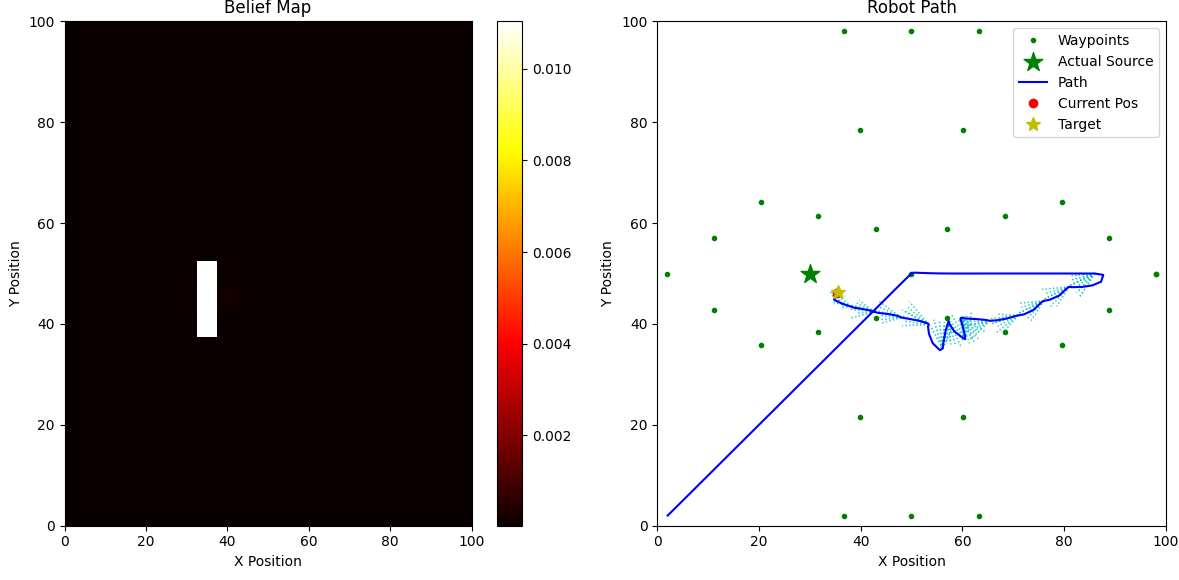
\includegraphics[width=\linewidth]{figures/rollout_algorithm.png}
        \caption{Rollout algorithm-based radiation source localization for source location (30, 50)}
        \label{fig:rollout_algorithm_plot}
    \end{figure}

    Figure~\ref{fig:rollout_algorithm_plot} represents the run of the rollout algorithm-based radiation source localization algorithm for a source located at (30, 50). The blue line represents 
    the path taken by the drone, the blue dotted line represents the trajectory rollouts from the current position, and the yellow start at the end of each algorithm chosen trajectory endpoint
    position. This run localized the source at a distance of 7 meters from the actual source location. 

    \subsubsection{Inverse Square Law Optimization}
    The implemented localization method is based on the inverse square law for radiation intensity and serves as a deterministic baseline for comparing different 
    radiation source search strategies. The algorithm employs a concentric search pattern that scales automatically according to the search area consisting of 
    three concentric circles positioned at 25\%, 50\%, and 75\% of the search area radius. This pattern begins from the center and expands outward, with the number 
    of measurement points per circle scaling proportionally with the map size to maintain consistent coverage across different search areas. The choice of using 
    concentric circles for data collection is based on tests showing that other patterns, such as shamrock, were less effective in terms of coverage and accuracy. 
    This approach balances the need to collect data covering most of the search space with the constraint of avoiding excessive time consumption.

        % The localization process relies on collecting radiation measurements at predefined points along this spiral trajectory. The source position estimation utilizes a weighted optimization 
        % approach incorporating the inverse square law, with higher weights assigned to stronger radiation readings to improve accuracy. To handle uncertainty in source intensity, the algorithm 
        % employs multiple optimization attempts with varying initial intensity estimates (100x, 1000x, and 10000x the maximum measured count rate) to avoid local minima. The uncertainty is further
        % quantified through a confidence circle around the estimated source position, with its radius proportional to the standard deviation of measurements. The uncertainty is further quantified 
        % through a confidence circle around the estimated source position, with its radius proportional to the standard deviation of measurements. The Nelder-Mead optimization method constrained 
        % to the defined search area processes these measurements to determine the most likely source position and intensity within bounded parameters.

    This method localizes the radiation source by beginning with deciding the search pattern and number of measurement points on this pattern scale based on the map size. At each
    measurement point, the radiation sensors collect radiation count and compare it against the expected measurements based on the inverse square law, which dictates that the intensity 
    decreases with the square distance from the source. These measurements are then weighted, assigning higher importance to stronger readings, as they indicate the proximity 
    to the source. The collected data is fed into the Nelder-Mead optimization algorithm, which iteratively adjusts the source position and intensity by minimizing the log-space error
    between the expected and measured radiation counts. To handle uncertainty in source intensity, the algorithm employs multiple optimization attempts with varying initial intensity estimates 
    (100x, 1000x, and 10000x the maximum measured count rate) to avoid local minima. The final estimated source position is accompanied by a confidence circle, whose radius is proportional to the 
    standard deviation of the measurements, indicating the uncertainty of the estimate.

        
    Many real-world problems involve objective functions that are not differentiable due to noise, discontinuities, and radiation measurements are one of those 
    problems. Gradient-based optimization methods struggle with such functions as they need smooth, differentiable functions to work. The Nelder-Mead algorithm is 
    effective for non-smooth or discontinuous functions because it does not rely on gradients. Instead, it evaluates the function at simplex vertices and adjusts the 
    simplex shape iteratively. This makes it a robust choice for optimization problems where derivative information is unavailable or unreliable. Compared to global optimization methods 
    like evolutionary algorithms, the Nelder-Mead approach offers lower computational costs for problems with fewer variables or limited evaluations, which aligns 
    well with the requirements of engineering optimization. \cite{luersen2004constrained}


    This approach is an effective baseline for comparison due to its deterministic nature, foundation in established physics principles, reproducible 
    behavior, and comprehensive evaluation metrics. The predefined path strategy and inverse square law optimization provide a methodical reference
    point against which more sophisticated, informed search strategies can be evaluated.
    
    \begin{figure}[ht]
        \centering
        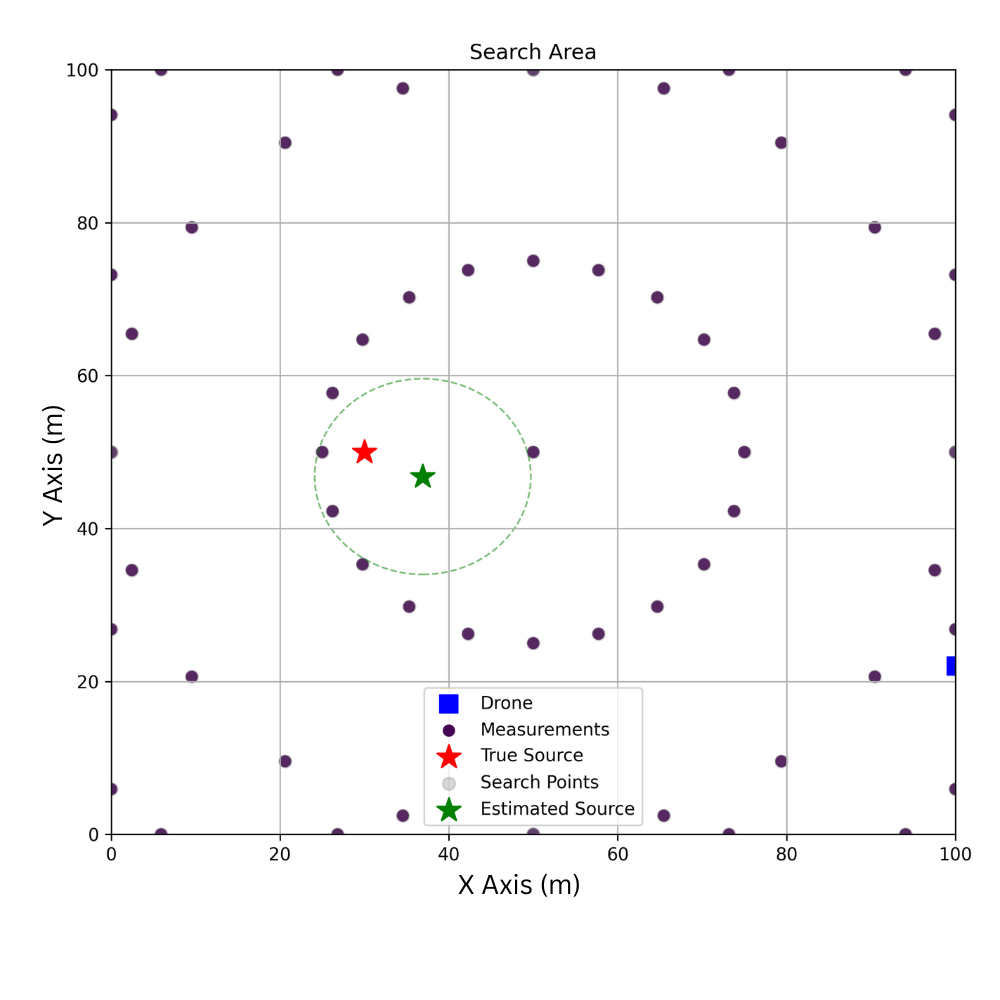
\includegraphics[width=\linewidth]{figures/inverse_square_method_with_label.png}
        \caption{inverse square optimization-based radiation source localization for source location (30, 50)}
        \label{fig:inverse_square_method_plot}
    \end{figure}

    Figure~\ref{fig:inverse_square_method_plot} represents the run of the inverse square law optimization-based radiation source localization algorithm for a source located at (30, 50). the green 
    ellipse represents the confidence circle around estimated source position(green star). The red star represents the true source position, black points represent the visited measurement points, and 
    the blue squre represents the estimated source position. This run localized the source at a distance of 7.6 meters from the actual source location.

    



\end{document}
